\documentclass[border=15pt]{standalone}
\usepackage{amsmath,amssymb,mathtools}
\usepackage{tikz}
\usepackage{pgfplots}
\usepackage{pgf}
\begin{document}
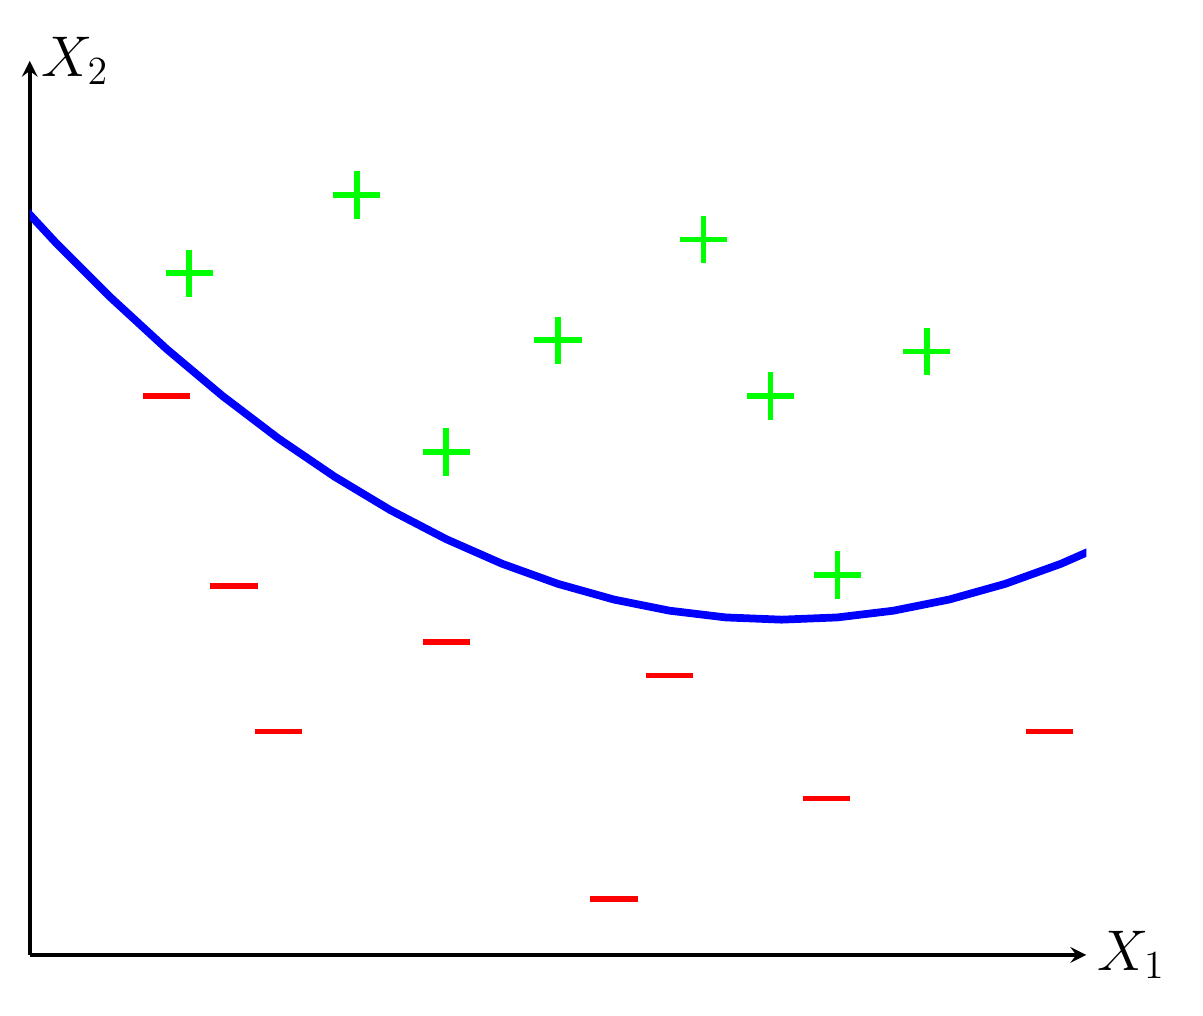
\begin{tikzpicture}
	\begin{axis}[
		xmin=1,
		xmax=9,
		ymin=1,
		ymax=9,
		axis equal,
		width=15cm,
		axis x line=center,
		axis y line=center,
		xmajorticks=false,
		ymajorticks=false,
		ylabel style={right,font=\huge},
		ylabel=$X_2$,
		xlabel style={above,right,font=\huge},
		xlabel=$X_1$,
		line width=1.5pt
		]
		%\addplot[no markers, domain=-1:11]{(5/3)*x};
		
		\addplot[only marks, mark=-,draw=red,mark size=0.3cm,line width=2pt]coordinates {(9.4, 3)
			(5.5 ,1.5)
			(1.5 ,6)
			(2.1 ,4.3)
			(2.5 ,3.0)
			( 4 ,3.8)
			(6,3.5)
			(7.4,2.4)};
		\addplot[only marks, mark=+,draw=green,mark size=0.3cm,line width=2pt]coordinates {
		(7.5, 4.4)
		(4,5.5)
		(6.3, 7.4)
		(5, 6.5)
		(8.3, 6.4)
		(1.7, 7.1)
		(3.2,7.8)
		(6.9,6)};
		\addplot[no markers,domain=-1:11,thick,blue,line width=2.8pt]{0.08*(x-7)^2+4};
	\end{axis}
\end{tikzpicture}
\end{document}